%\part{Konstruktion}
%\chapter{User Interface}

\section{ViewController}
Der ViewController dient zur Steuerung der Funktionen welche direkt mit dem Interface zusammen gehören. Dazu gehören
IBActions welche von Buttons oder anderen Interkationsflächen angestoßen werden können, sowie Funktionen welche direkt mit diesen zusammenhängen, Beziehungsweise aus diesen resultieren. Der ViewController ist die zweite Schicht nach dem UI. Im
Folgenden werden die einzelnen Viewcontroller mit ihren jeweiligen Funktionen beschrieben.
Der Viewcontroller ist der Hauptviewcontroller für die normale Browseransicht mit der Adresszeile und dem WkWebView. Er verwaltet die Kopzeile mit Adresszeile sowie den Buttons für Vorwärts, Zurück, Lesezeichen, Lesezeichen hinzufügen, Reload, Sech-Tabelle sowie die Settings. Die datei Main.js welche aus dem Viewcontroller heraus aufgerufen wird, markiert alle gefundenen Search-Tags. Außerdem wird im Falle eines Klicks die Position sowie die id des Search-Tags übermittelt.
Der PopViewController ist zuständig für die Verwaltung eines neuen PopViews, beim klicken auf einen Searchtag. Er verwaltet die Anzeige des ausgewählten Searchlinks in einem neuen WkWebView sowie den Button für die Auswahl der verschiedenen Suchergebnisse zu einem Searchtag.
Der SearchTableViewController verwaltet die einzellnen Suchergebnisse zu einem Searchtag. Alle Ergebnisse werden sortiert in einer Tabelle mit Bild, Title und Link angezeigt.
Der Settingscontroller is für die verwaltung der Browsereinstellungen zuständig.

\begin{figure}[ht]
	\centering
	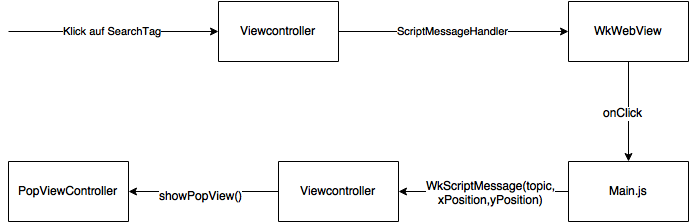
\includegraphics[width=\textwidth]{SearchTagAnzeige.png}
	\caption{Ablauf des Rankings}
	\label{fig:Searchtag Anzeige}
\end{figure}

Obige Grafik zeigt den Programmablauf beim Klick auf einen Searchtag. Die Postion des Klicks wird über JavaScript ausgelesen und an den WkWebview weitergeleitet. Dieser erzeugt ausgehend von der übertragenen Position einen PopView. 
\subsection{ViewController}
\subsection{SearchTableViewController}
\subsection{PopViewController}
\subsection{SettingsController}
\subsection{main.js}

%\subsubsection{Unterteilabschnitt}
%\paragraph{Paragraph}
%\subparagraph{Unterparagraph}
